% Options for packages loaded elsewhere
\PassOptionsToPackage{unicode}{hyperref}
\PassOptionsToPackage{hyphens}{url}
\PassOptionsToPackage{dvipsnames,svgnames,x11names}{xcolor}
%
\documentclass[
  8pt,
  a4paper]{article}

\usepackage{amsmath,amssymb}
\usepackage{iftex}
\ifPDFTeX
  \usepackage[T1]{fontenc}
  \usepackage[utf8]{inputenc}
  \usepackage{textcomp} % provide euro and other symbols
\else % if luatex or xetex
  \usepackage{unicode-math}
  \defaultfontfeatures{Scale=MatchLowercase}
  \defaultfontfeatures[\rmfamily]{Ligatures=TeX,Scale=1}
\fi
\usepackage{lmodern}
\ifPDFTeX\else  
    % xetex/luatex font selection
    \setmainfont[]{Arial}
    \setmonofont[]{DejaVu Sans Mono}
  \setmathfont[]{LiberationMono}
\fi
% Use upquote if available, for straight quotes in verbatim environments
\IfFileExists{upquote.sty}{\usepackage{upquote}}{}
\IfFileExists{microtype.sty}{% use microtype if available
  \usepackage[]{microtype}
  \UseMicrotypeSet[protrusion]{basicmath} % disable protrusion for tt fonts
}{}
\makeatletter
\@ifundefined{KOMAClassName}{% if non-KOMA class
  \IfFileExists{parskip.sty}{%
    \usepackage{parskip}
  }{% else
    \setlength{\parindent}{0pt}
    \setlength{\parskip}{6pt plus 2pt minus 1pt}}
}{% if KOMA class
  \KOMAoptions{parskip=half}}
\makeatother
\usepackage{xcolor}
\usepackage[lmargin=2cm,rmargin=2cm,tmargin=2cm,bmargin=2cm]{geometry}
\setlength{\emergencystretch}{3em} % prevent overfull lines
\setcounter{secnumdepth}{-\maxdimen} % remove section numbering
% Make \paragraph and \subparagraph free-standing
\makeatletter
\ifx\paragraph\undefined\else
  \let\oldparagraph\paragraph
  \renewcommand{\paragraph}{
    \@ifstar
      \xxxParagraphStar
      \xxxParagraphNoStar
  }
  \newcommand{\xxxParagraphStar}[1]{\oldparagraph*{#1}\mbox{}}
  \newcommand{\xxxParagraphNoStar}[1]{\oldparagraph{#1}\mbox{}}
\fi
\ifx\subparagraph\undefined\else
  \let\oldsubparagraph\subparagraph
  \renewcommand{\subparagraph}{
    \@ifstar
      \xxxSubParagraphStar
      \xxxSubParagraphNoStar
  }
  \newcommand{\xxxSubParagraphStar}[1]{\oldsubparagraph*{#1}\mbox{}}
  \newcommand{\xxxSubParagraphNoStar}[1]{\oldsubparagraph{#1}\mbox{}}
\fi
\makeatother


\providecommand{\tightlist}{%
  \setlength{\itemsep}{0pt}\setlength{\parskip}{0pt}}\usepackage{longtable,booktabs,array}
\usepackage{calc} % for calculating minipage widths
% Correct order of tables after \paragraph or \subparagraph
\usepackage{etoolbox}
\makeatletter
\patchcmd\longtable{\par}{\if@noskipsec\mbox{}\fi\par}{}{}
\makeatother
% Allow footnotes in longtable head/foot
\IfFileExists{footnotehyper.sty}{\usepackage{footnotehyper}}{\usepackage{footnote}}
\makesavenoteenv{longtable}
\usepackage{graphicx}
\makeatletter
\def\maxwidth{\ifdim\Gin@nat@width>\linewidth\linewidth\else\Gin@nat@width\fi}
\def\maxheight{\ifdim\Gin@nat@height>\textheight\textheight\else\Gin@nat@height\fi}
\makeatother
% Scale images if necessary, so that they will not overflow the page
% margins by default, and it is still possible to overwrite the defaults
% using explicit options in \includegraphics[width, height, ...]{}
\setkeys{Gin}{width=\maxwidth,height=\maxheight,keepaspectratio}
% Set default figure placement to htbp
\makeatletter
\def\fps@figure{htbp}
\makeatother
% definitions for citeproc citations
\NewDocumentCommand\citeproctext{}{}
\NewDocumentCommand\citeproc{mm}{%
  \begingroup\def\citeproctext{#2}\cite{#1}\endgroup}
\makeatletter
 % allow citations to break across lines
 \let\@cite@ofmt\@firstofone
 % avoid brackets around text for \cite:
 \def\@biblabel#1{}
 \def\@cite#1#2{{#1\if@tempswa , #2\fi}}
\makeatother
\newlength{\cslhangindent}
\setlength{\cslhangindent}{1.5em}
\newlength{\csllabelwidth}
\setlength{\csllabelwidth}{3em}
\newenvironment{CSLReferences}[2] % #1 hanging-indent, #2 entry-spacing
 {\begin{list}{}{%
  \setlength{\itemindent}{0pt}
  \setlength{\leftmargin}{0pt}
  \setlength{\parsep}{0pt}
  % turn on hanging indent if param 1 is 1
  \ifodd #1
   \setlength{\leftmargin}{\cslhangindent}
   \setlength{\itemindent}{-1\cslhangindent}
  \fi
  % set entry spacing
  \setlength{\itemsep}{#2\baselineskip}}}
 {\end{list}}
\usepackage{calc}
\newcommand{\CSLBlock}[1]{\hfill\break\parbox[t]{\linewidth}{\strut\ignorespaces#1\strut}}
\newcommand{\CSLLeftMargin}[1]{\parbox[t]{\csllabelwidth}{\strut#1\strut}}
\newcommand{\CSLRightInline}[1]{\parbox[t]{\linewidth - \csllabelwidth}{\strut#1\strut}}
\newcommand{\CSLIndent}[1]{\hspace{\cslhangindent}#1}

\makeatletter
\@ifpackageloaded{tcolorbox}{}{\usepackage[skins,breakable]{tcolorbox}}
\@ifpackageloaded{fontawesome5}{}{\usepackage{fontawesome5}}
\definecolor{quarto-callout-color}{HTML}{909090}
\definecolor{quarto-callout-note-color}{HTML}{0758E5}
\definecolor{quarto-callout-important-color}{HTML}{CC1914}
\definecolor{quarto-callout-warning-color}{HTML}{EB9113}
\definecolor{quarto-callout-tip-color}{HTML}{00A047}
\definecolor{quarto-callout-caution-color}{HTML}{FC5300}
\definecolor{quarto-callout-color-frame}{HTML}{acacac}
\definecolor{quarto-callout-note-color-frame}{HTML}{4582ec}
\definecolor{quarto-callout-important-color-frame}{HTML}{d9534f}
\definecolor{quarto-callout-warning-color-frame}{HTML}{f0ad4e}
\definecolor{quarto-callout-tip-color-frame}{HTML}{02b875}
\definecolor{quarto-callout-caution-color-frame}{HTML}{fd7e14}
\makeatother
\makeatletter
\@ifpackageloaded{caption}{}{\usepackage{caption}}
\AtBeginDocument{%
\ifdefined\contentsname
  \renewcommand*\contentsname{Table of contents}
\else
  \newcommand\contentsname{Table of contents}
\fi
\ifdefined\listfigurename
  \renewcommand*\listfigurename{List of Figures}
\else
  \newcommand\listfigurename{List of Figures}
\fi
\ifdefined\listtablename
  \renewcommand*\listtablename{List of Tables}
\else
  \newcommand\listtablename{List of Tables}
\fi
\ifdefined\figurename
  \renewcommand*\figurename{\textbf{Figure}}
\else
  \newcommand\figurename{\textbf{Figure}}
\fi
\ifdefined\tablename
  \renewcommand*\tablename{\textbf{Table}}
\else
  \newcommand\tablename{\textbf{Table}}
\fi
}
\@ifpackageloaded{float}{}{\usepackage{float}}
\floatstyle{ruled}
\@ifundefined{c@chapter}{\newfloat{codelisting}{h}{lop}}{\newfloat{codelisting}{h}{lop}[chapter]}
\floatname{codelisting}{Listing}
\newcommand*\listoflistings{\listof{codelisting}{List of Listings}}
\makeatother
\makeatletter
\makeatother
\makeatletter
\@ifpackageloaded{caption}{}{\usepackage{caption}}
\@ifpackageloaded{subcaption}{}{\usepackage{subcaption}}
\makeatother
\makeatletter
\@ifpackageloaded{fontawesome5}{}{\usepackage{fontawesome5}}
\makeatother

\ifLuaTeX
  \usepackage{selnolig}  % disable illegal ligatures
\fi
\usepackage{bookmark}

\IfFileExists{xurl.sty}{\usepackage{xurl}}{} % add URL line breaks if available
\urlstyle{same} % disable monospaced font for URLs
\hypersetup{
  pdftitle={Darwin Harbour sediment monitoring program analysis application manual},
  pdfauthor={Murray Logan},
  colorlinks=true,
  linkcolor={blue},
  filecolor={Maroon},
  citecolor={Blue},
  urlcolor={Blue},
  pdfcreator={LaTeX via pandoc}}


\title{Darwin Harbour sediment monitoring program analysis application
manual}
\author{Murray Logan}
\date{12/07/2024}

\begin{document}
\maketitle

\renewcommand*\contentsname{Table of contents}
{
\hypersetup{linkcolor=}
\setcounter{tocdepth}{3}
\tableofcontents
}

\section{About}\label{about}

This document comprises the manual for the Darwin Harbour sediment
monitoring program analysis application. It provides information on:

\begin{itemize}
\tightlist
\item
  a broad overview of the structure of the application
\item
  the application dependencies and how to install them
\item
  starting the application
\item
  progressing through the analysis pipeline
\item
  visualising, interpreting and extracting outputs
\end{itemize}

\section{Structural overview}\label{structural-overview}

\href{https://www.r-project.org/}{R Graphical and Statistical
Environment} offers an ideal platform for developing and running complex
statistical analyses as well as presenting the outcomes via professional
graphical/tabular representations. As a completely scripted language it
also offers the potential for both full transparency and
reproducibility. Nevertheless, as the language, and more specifically
the extension packages are community developed and maintained, the
environment evolves over time. Similarly, the underlying operating
systems and programs on which R and its extension packages depend
(hereafter referred to as the \emph{operating environment}) also change
over time. Consequently, the stability and reproducibility of R codes
have a tendency to change over time.

\subsection{Docker containers}\label{docker-containers}

One way to attempt to future proof a codebase that must be run upon a
potentially unpredictable operating environment is to
\textbf{containerise} the operating environment, such that it is
preserved to remain unchanged over time. Containers (specifically
\href{https://www.docker.com/}{docker} containers) are lightweight
abstraction units that encapsulate applications and their dependencies
within standardized, self-contained execution environments. Leveraging
containerization technology, they package application code, runtime,
libraries, and system tools into isolated units (\emph{containers}) that
abstract away underlying infrastructure differences, enabling consistent
and predictable execution across diverse computing platforms.

Containers offer several advantages, such as efficient resource
utilization, rapid deployment, and scalability. They enable developers
to build, test, and deploy applications with greater speed and
flexibility. Docker containers have become a fundamental building block
in modern software development, enabling the development and deployment
of applications in a consistent and predictable manner across various
environments.

\subsection{Shiny applications}\label{shiny-applications}

\href{https://shiny.posit.co/}{Shiny} is a web application framework for
R that enables the creation of interactive and data-driven web
applications directly from R scripts. Developed by
\href{https://posit.co/}{Rstudio}, Shiny simplifies the process of
turning analyses into interactive web-based tools without the need for
extensive web development expertise.

What makes Shiny particularly valuable is its seamless integration with
R, allowing statisticians and data scientists to build and deploy
bespoke statistical applications, thereby making data visualization,
exploration, and analysis accessible to a broader audience. With its
interactive and user-friendly nature, Shiny serves as a powerful tool
for sharing insights and engaging stakeholders in a more intuitive and
visual manner.

\subsection{Git and github}\label{git-and-github}

Git, a distributed version control system, and
\href{https://github.com/}{GitHub}, a web-based platform for hosting and
collaborating on Git repositories, play pivotal roles in enhancing
reproducibility and transparency in software development. By tracking
changes in source code and providing a centralized platform for
collaborative work, Git and GitHub enable developers to maintain a
detailed history of code alterations. This history serves as a valuable
asset for ensuring the reproducibility of software projects, allowing
users to trace and replicate specific versions of the codebase.

GitHub Actions (an integrated workflow automation feature of GitHub),
automates tasks such as building, testing, and deploying applications
and artifacts. Notably, through workflow actions, GitHub Actions can
build docker containers and act as a container registry. This
integration enhances the overall transparency of software development
workflows, making it easier to share, understand, and reproduce projects
collaboratively.

Figure~\ref{fig-diagram} provides a schematic overview of the
relationship between the code produced by the developer, the Github
cloud repositiory and container registry and the shiny docker container
run by user.

\begin{figure}

\centering{

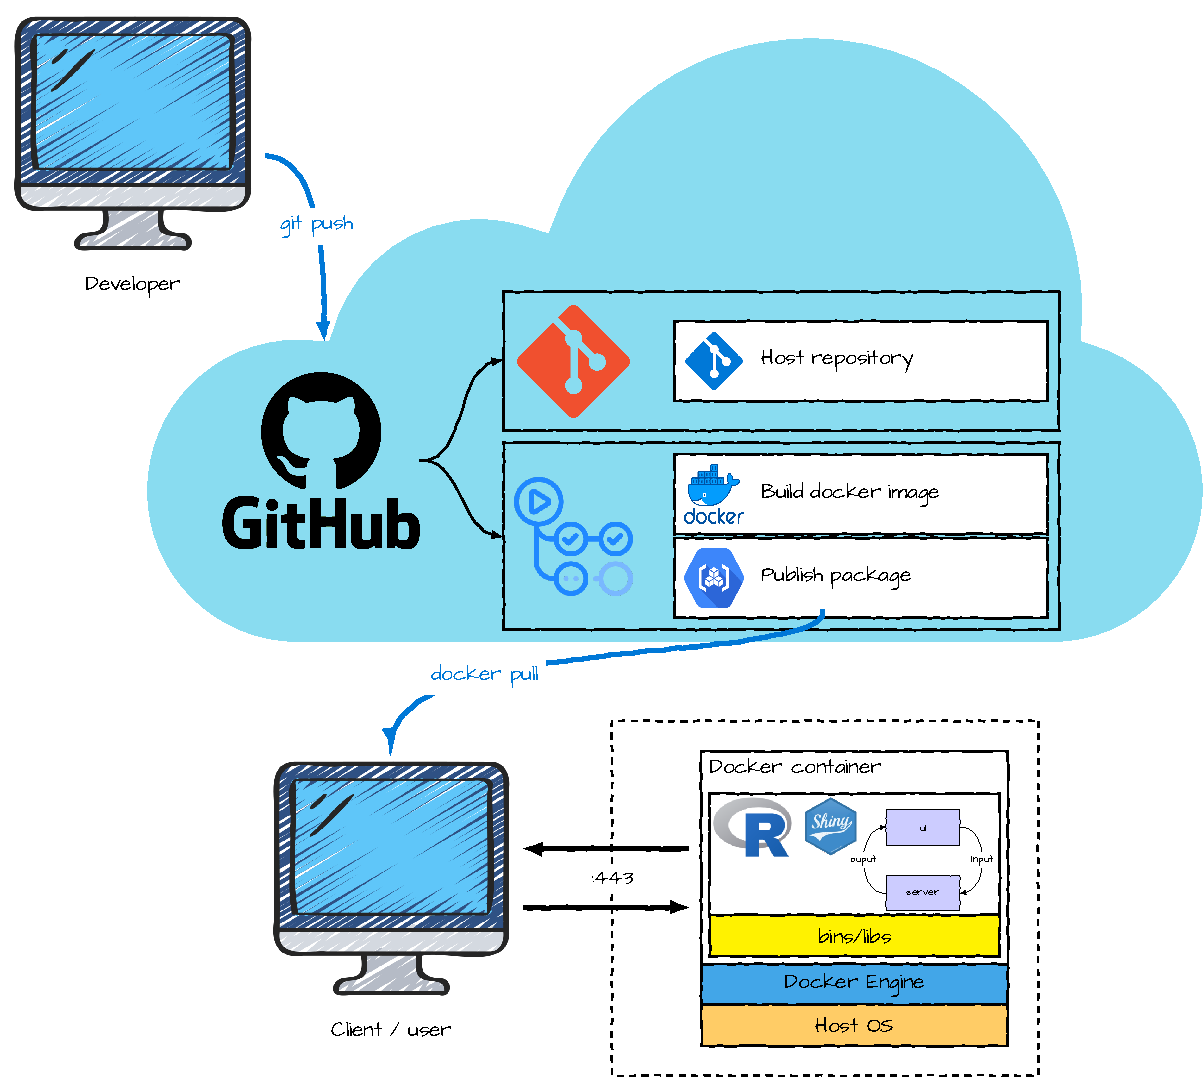
\includegraphics{manual_files/figure-pdf/fig-diagram-1.pdf}

}

\caption{\label{fig-diagram}Diagram illustrating the relationship
between the code produced by the developer and the shiny docker
container utilised by user with a Github cloud conduit. The developed
codebase includes a Shiny R application with R backend,
\texttt{Dockerfile} (instructions used to assemble a full operating
environment) and github workflow file (instructions for building and
packaging the docker image on github via \texttt{actions}).}

\end{figure}%

\section{Installation}\label{installation}

\subsection{Installing docker desktop}\label{installing-docker-desktop}

To retrieve and run docker containers requires the installation of
\href{https://www.docker.com/products/docker-desktop/}{Docker Desktop}
on Windows and MacOSx

\subsubsection{Windows}\label{windows}

The steps for installing Docker Desktop are:

\begin{itemize}
\item
  \textbf{Download the Installer:} head to
  \url{https://docs.docker.com/desktop/install/windows-install/} and
  follow the instructions for downloading the appropriate installer for
  your Windows version (Home or Pro).
\item
  \textbf{Run the Installer:} double-click the downloaded file and
  follow the on-screen instructions from the installation wizard. Accept
  the license agreement and choose your preferred installation location.
\item
  \textbf{Configure Resources (Optional):} Docker Desktop might suggest
  allocating some system resources like CPU and memory. These settings
  can be adjusted later, so feel free to use the defaults for now.
\item
  \textbf{Start the Docker Engine:} once installed, click the ``Start
  Docker Desktop'' button. You may see a notification in the taskbar -
  click it to confirm and allow Docker to run in the background.
\item
  \textbf{Verification:} open a terminal (or Powershell) and run
  \texttt{docker\ -\/-version}. If all went well, you should see
  information about the installed Docker Engine version.
\end{itemize}

Additional Tips:

\begin{itemize}
\tightlist
\item
  Ensure Hyper-V (virtualization) is enabled in your BIOS settings for
  optimal performance.
\end{itemize}

\subsection{Installing the and running the
app}\label{installing-the-and-running-the-app}

The task of installing and running the app is performed via a single
\textbf{deploy script} (\texttt{deploy.bat} on Windows or
\texttt{deploy.sh} on Linux/MacOSX/wsl). For this to work properly, the
deploy script should be placed in a folder along with a folder (called
\texttt{input}) that contains the input datasets (in excel format). This
structure is illustrated below for Windows.

\begin{verbatim}
\
|- deploy.bat
|- input
   |- dataset1.xlsx
   |- dataset2.xlsx
\end{verbatim}

\begin{tcolorbox}[enhanced jigsaw, toprule=.15mm, opacityback=0, colbacktitle=quarto-callout-note-color!10!white, colback=white, breakable, opacitybacktitle=0.6, toptitle=1mm, colframe=quarto-callout-note-color-frame, title=\textcolor{quarto-callout-note-color}{\faInfo}\hspace{0.5em}{Note}, rightrule=.15mm, leftrule=.75mm, bottomrule=.15mm, left=2mm, bottomtitle=1mm, coltitle=black, titlerule=0mm, arc=.35mm]

In the above illustration, there are two example datasets
(\texttt{dataset1.xlsx} and \texttt{dataset2.xlsx}). The datasets need
NOT be called \texttt{dataset1.xlsx}. They can have any name you choose,
so long as they are excel files that adhere to the structure outlined in
Section~\ref{sec-data-requirements}.

\end{tcolorbox}

To set up the above struture:

\begin{enumerate}
\def\labelenumi{\arabic{enumi}.}
\item
  create a new folder on your computer in a location of your choice that
  you are likely to remember and easily locate (e.g.~on the desktop).
  Whilst the name of the folder is not important, it is recommended that
  it be named after the project (e.g.
  \texttt{darwin\_harbour\_sediment\_monitoring}).
\item
  download the deploy script from the projects github repository

  \begin{enumerate}
  \def\labelenumii{\alph{enumii}.}
  \item
    go to the projects github repository
    (\url{https://github.com/open-AIMS/dh_sediment_monitoring.git}) in a
    browser
  \item
    click on either the \texttt{deploy.bat} (Windows) or 'deploy.sh`
    (Linux/MacOSX/wsl).

    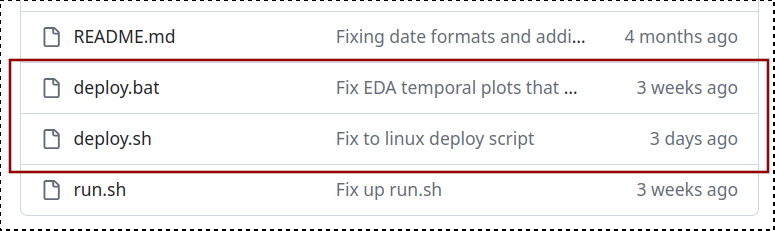
\includegraphics{resources/github_deploy_script.png}
  \item
    click on the download button and select the project folder as the
    location to download the file to. If the file is automatically
    downloaded to a downloads folder, move the file to the project
    folder.

    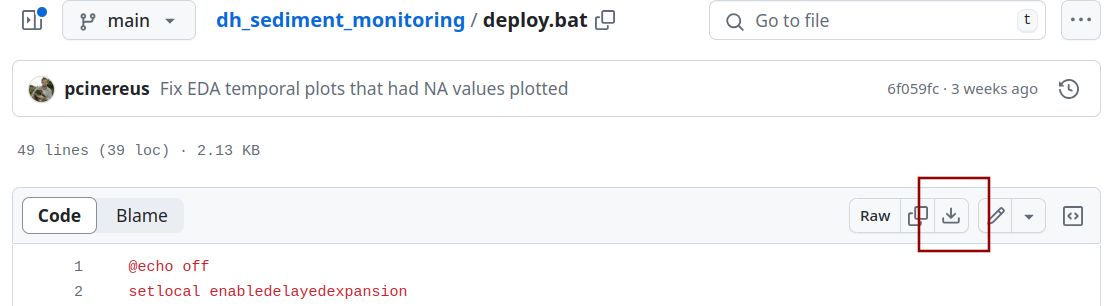
\includegraphics{resources/github_deploy_script2.png}
  \end{enumerate}
\item
  within the project folder, create a folder called \texttt{inputs} and
  place all the appropriate data sets into this \texttt{inputs} folder
\end{enumerate}

To run the app, navigate inside of the project folder and run (typically
double click) on the deploy script. Upon doing so, you will be presented
with a directory selection window that is prompting for the path of the
project folder. Navigate to and select the project folder before
clicking the ``OK'' button. Shortly thereafter, the application will
appear in a browser tab.

\begin{tcolorbox}[enhanced jigsaw, toprule=.15mm, opacityback=0, colbacktitle=quarto-callout-note-color!10!white, colback=white, breakable, opacitybacktitle=0.6, toptitle=1mm, colframe=quarto-callout-note-color-frame, title=\textcolor{quarto-callout-note-color}{\faInfo}\hspace{0.5em}{More specific information about the \texttt{deploy.bat} script}, rightrule=.15mm, leftrule=.75mm, bottomrule=.15mm, left=2mm, bottomtitle=1mm, coltitle=black, titlerule=0mm, arc=.35mm]

The \texttt{deploy.bat} script performs the following:

\begin{enumerate}
\def\labelenumi{\arabic{enumi}.}
\tightlist
\item
  defines paths to the project repository and local project folder
\item
  checks if \texttt{docker} is installed and available from the command
  line for the current user
\item
  checks if \texttt{docker} is running
\item
  query the user for the location of the project folder
\item
  determine whether there are any updates to the \texttt{docker} image
  and if so pull them down
\item
  run the \texttt{docker} container
\item
  open the shiny app in a browser
\end{enumerate}

\end{tcolorbox}

\section{The Darwin Harbour Sediment Monitoring Program Analysis
App}\label{the-darwin-harbour-sediment-monitoring-program-analysis-app}

This \href{https://shiny.posit.co/}{Shiny} application is designed to
ingest very specifically structured excel spreadsheets containing Darwin
Harbour sediment monitoring data and produce various analyses and
visualisations. The application is served from a
\href{https://www.docker.com/}{docker} container to the localhost and
the default web browser.

Docker containers can be thought of a computers running within other
computers. More specifically, a container runs an instance of image
built using a series of specific instructions that govern the entire
software environment. As a result, containers run from the same image
will operate (virtually) identically regardless of the host environment.
Furthermore, since the build instructions can specify exact versions of
all software components, containers provide a way of maximising the
chances that an application will continue to run as designed into the
future despite changes to operating environments and dependencies.

This shiny application comprises five pages (each accessable via the
sidebar menu on the left side of the screen):

\begin{enumerate}
\def\labelenumi{\arabic{enumi}.}
\tightlist
\item
  a \textbf{Landing} page (this page) providing access to the settings
  and overall initial instructions
\item
  a \textbf{Dashboard} providing information about the progression of
  tasks in the analysis pipeline
\item
  a \textbf{Data} page providing overviews of data in various stages
\item
  an \textbf{Exploratory Data Analysis} page providing graphical data
  summaries
\item
  an \textbf{Analysis} page providing information about the statistical
  models and their outputs
\item
  a \textbf{Manual} page that displays the online manual for the
  application
\end{enumerate}

Each page will also contain instructions to help guide you through using
or interpreting the information. In some cases, this will take the from
of an info box (such as the current box). In other cases, it will take
the form of little {} symbols whose content is revealed with a mouse
hover.

There are numerous stages throughout the analysis pipeline that may
require user review (for example examining the exploratory data analysis
figures to confirm that the data are as expected). Consequently, it is
necessary for the user to manually trigger each successive stage of the
pipeline. The stages are:

\begin{itemize}
\item
  Stage 1 - Prepare environment

  More info

  This stage is run automatically on startup and essentially sets up the
  operating environment.
\item
  Stage 2 - Obtain data

  More info

  This stage comprises of the following steps:

  \begin{itemize}
  \tightlist
  \item
    reading in the excel files within the nominated input path
  \item
    validating the input data according to a set of validation rules
  \item
    constructing various spatial objects for mapping and spatial
    aggregation purposes
  \end{itemize}

  The tables within the \textbf{Raw data} tab of the \textbf{Data} page
  will also be populated.
\item
  Stage 3 - Process data

  More info

  This stage comprises of the following steps:

  \begin{itemize}
  \tightlist
  \item
    apply limit of reporing values (LoRs)
  \item
    pivot the data into a longer format that is more suitable for
    analysis and graphing
  \item
    join in the metadata to each associated sheet
  \item
    make a unique key
  \item
    collate the all the data together from across the multiple sheets
    and files into a single data set
  \item
    incorporate the spatial data
  \item
    tidy the field names
  \item
    apply data standardisations
  \item
    create a site lookup table to facilitate fast incorporation of
    spatial information into any outputs.
  \end{itemize}

  The tables within the \textbf{Processed data} tab of the \textbf{Data}
  page will also be populated.
\item
  Stage 4 - Exploratory data analysis

  More info

  This stage comprises of the following steps:

  \begin{itemize}
  \tightlist
  \item
    retrieve the processed data.
  \item
    construct spatio-temporal design plots conditioned on initial
    sampling semester
  \item
    construct variable temporal design plots conditioned on harbour zone
  \item
    construct site level temporal trends for each variable
  \item
    construct zone level temporal and spatial visualisations for each
    variable
  \end{itemize}

  The exploratory data figures of the \textbf{Exploratory Data Analysis}
  page will also be populated.
\item
  Stage 5 - Temporal analyses

  More info

  This stage comprises of the following steps:

  \begin{itemize}
  \tightlist
  \item
    retrieve the processed data
  \item
    prepare the data for modelling
  \item
    prepare appropriate model formulae for each zone, variable,
    standardisation type
  \item
    prepare appropriate model priors for each zone, variable,
    standardisation type
  \item
    prepare appropriate model template
  \item
    fit the models for each zone, variable, standardisation type
  \item
    perform model validations for each zone, variable, standardisation
    type
  \item
    estimate all the contrasts for each model and collate all the
    effects
  \end{itemize}
\end{itemize}

Underneath the sidebar menu there are a series of buttons that control
progression through the analysis pipeline stages. When a button is blue
(and has a play icon), it indicates that the Stage is the next Stage to
be run in the pipeline. Once a stage has run, the button will turn
green. Grey buttons are disabled.

Clicking on button will run that stage. Once a stage has run, the button
will change to either green (success), yellow (orange) or red (failures)
indicating whether errors/warnings were encountered or not. If the stage
was completed successfully, the button corresponding to the next
available stage will be activated.

Sidebar menu items that are in orange font are active and clicking on an
active menu item will reveal an associated page. Inactive menu items are
in grey font. Menu items will only become active once the appropriate
run stage has been met. The following table lists the events that
activate a menu item.

\begin{longtable}[]{@{}ll@{}}
\toprule\noalign{}
Menu Item & Trigger Event \\
\midrule\noalign{}
\endhead
\bottomrule\noalign{}
\endlastfoot
Landing & Always active \\
Dashboard & Always active \\
Data & After Stage 2 \\
Exploratory Data Analysis & After Stage 4 \\
Analysis & After Stage 5 \\
Manual & Always active \\
\end{longtable}

Figure~\ref{fig-diagram2} provides a schematic overview the sequence of
filesystem events that occur during the development, deployment and
running of this app.

\begin{enumerate}
\def\labelenumi{\arabic{enumi}.}
\tightlist
\item
  the developed codebase is pushed to github and if necessary continuous
  integration (github actions) is triggered. The continuous integration
  will re-build and host a docker image as well as rebuild the manual.
\item
  when the client runs the \texttt{deploy.bat} (or \texttt{deploy.sh})
  script, it will check whether docker is running and get input from the
  user about the location of the project directory.
\item
  github will be queried to discover if a new docker image is available.
  If so, then the new image will be pulled down locally and run (if
  docker is runnning).
\item
  the docker container will be run and this will trigger git within the
  container to pull down the latest version of the codebase from github
  to a temporary repo in the container. As the container is starting up,
  it will mount the project folder so that its contents are available to
  the environment within container and outputs produced within the
  container are available to the host.
\item
  some of the files in the temporary repo will be copied to a folder
  within the project folder.
\item
  the shiny app will start up on \texttt{port\ 3838} of the localhost
  and this will be offered to the default browser.
\item
  as the shiny app progresses through each of the analysis stages, more
  data will be added to various folders of the project directory.
\end{enumerate}

\begin{figure}

\centering{

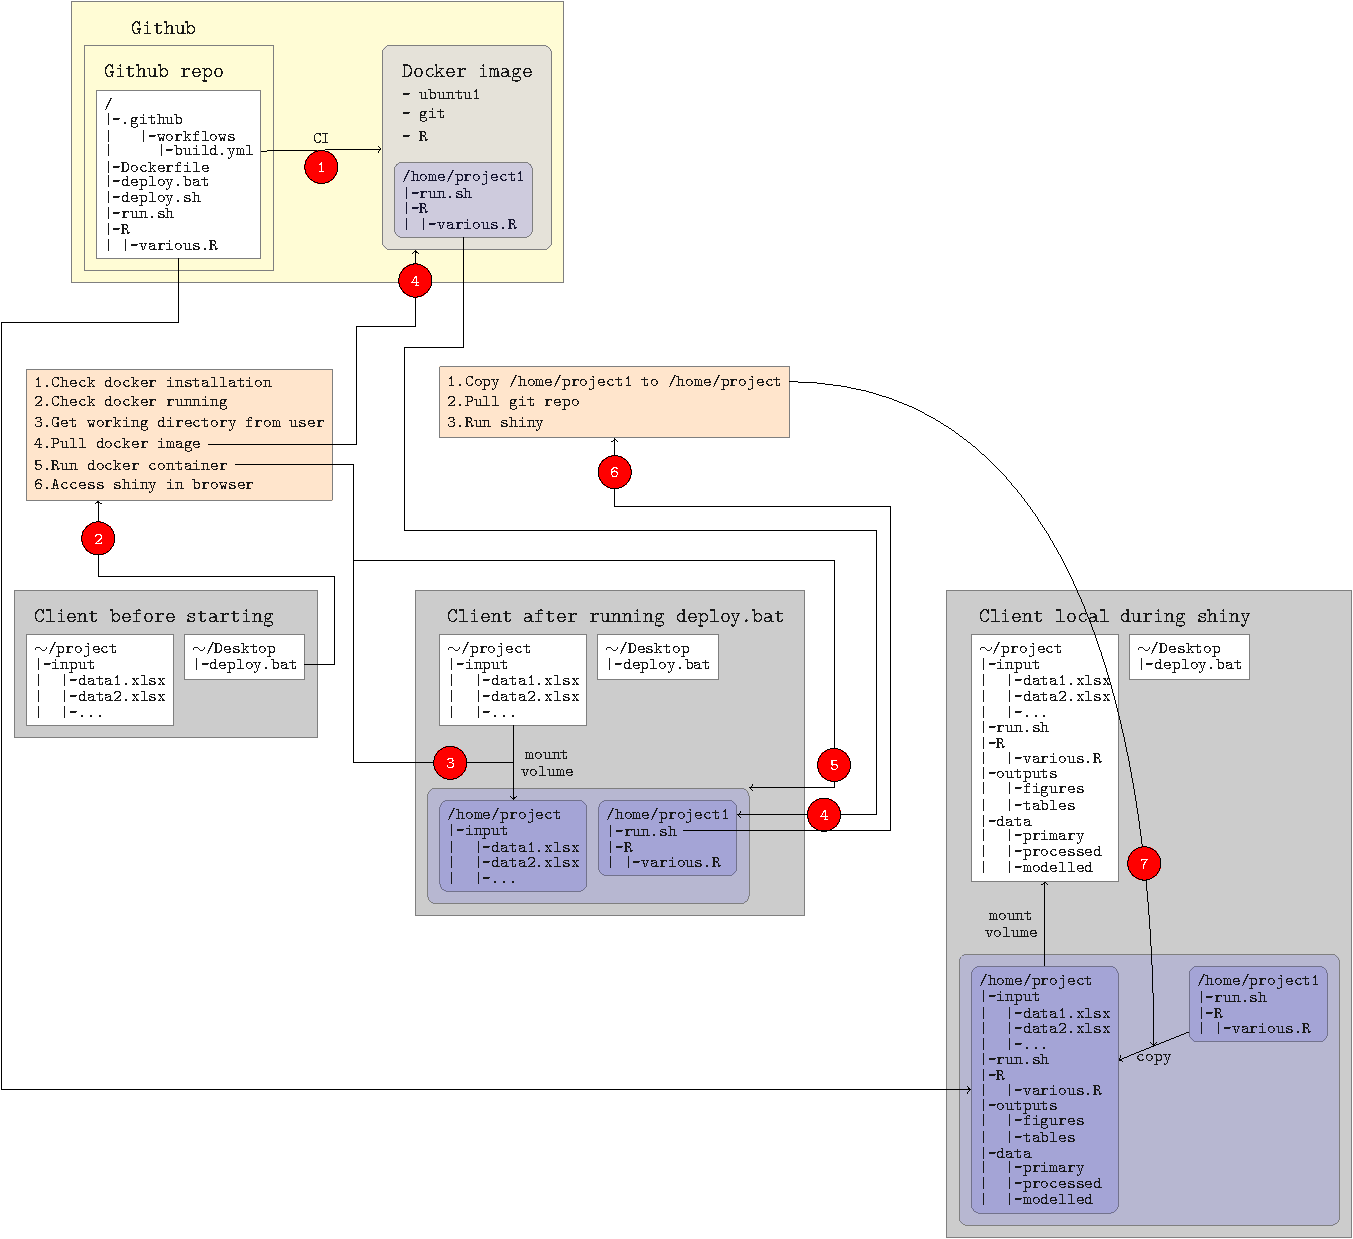
\includegraphics{manual_files/figure-pdf/fig-diagram2-1.pdf}

}

\caption{\label{fig-diagram2}Diagram illustrating the sequence of
filesystem events that occur during the development, deployment and
running of this app.}

\end{figure}%

\section{Analysis stages}\label{analysis-stages}

\subsection{Stage 2 - obtaining the
data}\label{stage-2---obtaining-the-data}

At the completion of this stage, the Data sidebar menu and Stage 3
button will become active and the Data page will be populated with the
raw data and available for review.

\subsubsection{Read input info}\label{read-input-info}

This task seeks to determine what data sources are available and for
those found, stores the names and filetypes discovered. This task will
exclusively search in the \texttt{/input} folder of the project
directory.

\subsubsection{Read input data}\label{read-input-data}

This task will sequentially read in each sheet of each data source
(excel file) into a nested list.

\subsubsection{Fix dates}\label{fix-dates}

This task will ensure that all dates are of the same format.
Spreadsheets often store date/time data in one format and display it in
another format. Consequently, users can be unaware that they have a
mixture of date/time formats present in the same spreadsheet. For the
purpose of data analysis, it is important that all date/time formats are
consistent - this task aims to achieve this.

\subsubsection{Validate input data}\label{validate-input-data}

This task performs data validation in accordance with the rules set out
in the following section.

\paragraph{Data requirements}\label{sec-data-requirements}

To be valid, input data must be excel files (*.xlsx) comprising at least
the following sheets (each of which must at least have the fields listed
in their respective tables):

\begin{itemize}
\item
  metals

  \begin{longtable}[]{@{}
    >{\raggedright\arraybackslash}p{(\columnwidth - 4\tabcolsep) * \real{0.1017}}
    >{\raggedright\arraybackslash}p{(\columnwidth - 4\tabcolsep) * \real{0.4407}}
    >{\raggedright\arraybackslash}p{(\columnwidth - 4\tabcolsep) * \real{0.4576}}@{}}
  \toprule\noalign{}
  \begin{minipage}[b]{\linewidth}\raggedright
  Field
  \end{minipage} & \begin{minipage}[b]{\linewidth}\raggedright
  Description
  \end{minipage} & \begin{minipage}[b]{\linewidth}\raggedright
  Validation conditions
  \end{minipage} \\
  \midrule\noalign{}
  \endhead
  \bottomrule\noalign{}
  \endlastfoot
  Sample\_ID & unique sample ID & must contain characters \\
  *¹ (mg/kg) & observed concentration of metal in sediment sample & must
  contain only numbers or start with a `\textless{}' symbol \\
  \end{longtable}

  1: where the '*' represents a one or two character chemical symbol
  (such as `Ag' or `V'). There should be numerous of these fields
\item
  hydrocarbons

  \begin{longtable}[]{@{}
    >{\raggedright\arraybackslash}p{(\columnwidth - 4\tabcolsep) * \real{0.1000}}
    >{\raggedright\arraybackslash}p{(\columnwidth - 4\tabcolsep) * \real{0.5000}}
    >{\raggedright\arraybackslash}p{(\columnwidth - 4\tabcolsep) * \real{0.4000}}@{}}
  \toprule\noalign{}
  \begin{minipage}[b]{\linewidth}\raggedright
  Field
  \end{minipage} & \begin{minipage}[b]{\linewidth}\raggedright
  Description
  \end{minipage} & \begin{minipage}[b]{\linewidth}\raggedright
  Validation conditions
  \end{minipage} \\
  \midrule\noalign{}
  \endhead
  \bottomrule\noalign{}
  \endlastfoot
  Sample\_ID & unique sample ID & must contain characters \\
  \textgreater C*¹ & observed concentration of hydrocarbons within a
  specific size bin in sediment sample & must contain only numbers or
  start with a `\textless{}' symbol \\
  \end{longtable}

  1: where the '*' represents a string of characters defining the size
  bin (such as '10 \_C16'). There should be numerous of these fields
\item
  total\_carbons

  \begin{longtable}[]{@{}
    >{\raggedright\arraybackslash}p{(\columnwidth - 4\tabcolsep) * \real{0.1000}}
    >{\raggedright\arraybackslash}p{(\columnwidth - 4\tabcolsep) * \real{0.5000}}
    >{\raggedright\arraybackslash}p{(\columnwidth - 4\tabcolsep) * \real{0.4000}}@{}}
  \toprule\noalign{}
  \begin{minipage}[b]{\linewidth}\raggedright
  Field
  \end{minipage} & \begin{minipage}[b]{\linewidth}\raggedright
  Description
  \end{minipage} & \begin{minipage}[b]{\linewidth}\raggedright
  Validation conditions
  \end{minipage} \\
  \midrule\noalign{}
  \endhead
  \bottomrule\noalign{}
  \endlastfoot
  Sample\_ID & unique sample ID & must contain characters \\
  TOC (\%) & observed total organic carbon (as a percentage of the
  sample weight) & must contain only numbers \\
  \end{longtable}
\item
  metadata

  \begin{longtable}[]{@{}
    >{\raggedright\arraybackslash}p{(\columnwidth - 4\tabcolsep) * \real{0.2500}}
    >{\raggedright\arraybackslash}p{(\columnwidth - 4\tabcolsep) * \real{0.3500}}
    >{\raggedright\arraybackslash}p{(\columnwidth - 4\tabcolsep) * \real{0.4000}}@{}}
  \toprule\noalign{}
  \begin{minipage}[b]{\linewidth}\raggedright
  Field
  \end{minipage} & \begin{minipage}[b]{\linewidth}\raggedright
  Description
  \end{minipage} & \begin{minipage}[b]{\linewidth}\raggedright
  Validation conditions
  \end{minipage} \\
  \midrule\noalign{}
  \endhead
  \bottomrule\noalign{}
  \endlastfoot
  IBSM\_site & name of the site from the perspective of IBSM & must
  contain characters (or be blank) \\
  Site\_ID & a unique site ID & must contain characters (cannot be
  blank) \\
  Sample\_ID & unique sample ID (the key to data sheets) & must contain
  characters (cannot be blank) \\
  Original\_SampleID & unique sample ID & must contain characters \\
  Latitude & site latitude & must be numeric (and negative) \\
  Longitude & site longitude & must be numeric \\
  Acquire\_date\_time & date and time sample was collected (D/M/YYYY
  hh:mm:ss) & must be in datetime format \\
  Sampler & name of person responsible for collecting sample (ignored) &
  ignored \\
  Notes & project description (ignored) & ignored \\
  Baseline\_site & the unique site ID of the corresponding baseline
  sample & must contain characters (cannot be blank) \\
  Baseline\_acquire\_date\_site & the date and time of the corresponding
  baseline sample & must be in datetime format \\
  \end{longtable}
\item
  notes - this sheet is not processed or validated
\end{itemize}

\begin{tcolorbox}[enhanced jigsaw, toprule=.15mm, opacityback=0, colbacktitle=quarto-callout-note-color!10!white, colback=white, breakable, opacitybacktitle=0.6, toptitle=1mm, colframe=quarto-callout-note-color-frame, title=\textcolor{quarto-callout-note-color}{\faInfo}\hspace{0.5em}{Note}, rightrule=.15mm, leftrule=.75mm, bottomrule=.15mm, left=2mm, bottomtitle=1mm, coltitle=black, titlerule=0mm, arc=.35mm]

All input data must be placed in the \texttt{/input} folder of the
Project prior to starting the app.

\end{tcolorbox}

\subsubsection{Make spatial data}\label{make-spatial-data}

This task will compile a set of spatial artifacts from GIS shapefiles of
Darwin Harbour. These spatial artifacts will be used to spatially join
the sediment data in order to assign spatial scales such as Zones and
Areas to the data. They will also be used to facilitate mapping of the
data. The shapefiles used in this task are built into the app. If there
is a need to change these, please contact the app author.

\subsubsection{Make spatial lookup}\label{make-spatial-lookup}

This stage creates a lookup table that relates each of the spatial
scales to one another. This lookup is used to inject the spatial
information into the data and modelled derivatives after they are
created and in so doing prevents the need to spatially join the data
each time it is required.

\subsection{Stage 3 - processing the
data}\label{stage-3---processing-the-data}

At the completion of this stage, the Stage 4 button will become active
and the Processed Data sub-page of the Data page will be populated with
the processed data and available for review.

\subsubsection{Retrieve data}\label{retrieve-data}

This task literally just reads in the data stored at the end of the
previous stage.

\subsubsection{Apply LoRs}\label{apply-lors}

This task applies rules for the presence of data that are below Limit of
Reporting (LoR). In the data, LoR values are indicated by the presence
of a \texttt{\textless{}} symbol. There are two ways available for
handling LoR values.

\begin{enumerate}
\def\labelenumi{\arabic{enumi}.}
\tightlist
\item
  Traditionally, values that represent Limit of Reporting (LoR) were
  replaced with half the LoR value. For example, a value of
  \textless0.02 would be replaced with 0.01.
\item
  However, modern statistical analyses have more appropriate ways of
  incorporating LoR information. Rather than arbitrarily replace values
  with half the LoR, we retain their value and flag them as censored and
  allow the statistical properties of disbutions to handle them more
  naturally.
\end{enumerate}

In either case, a LoR flag is then attached to any value that was deemed
LoR.

\subsubsection{Pivot data}\label{pivot-data}

This task pivots (reshapes) the data from wide to long format. Wide
format, in which each row represents a single site/time and each
variable is in its own column is a convenient way to assemble data
(particularly as it permits the user to easily identify missing values).
However, data analysis requires that each individual record
(observation) be in its own row.

\subsubsection{Join metadata}\label{join-metadata}

This task joins (merges) the each of the main sediment data sheets
(metals, hydrocarbons and total carbons) with the metadata sheet.

\subsubsection{Make sample key}\label{make-sample-key}

This task generates a unique key to uniquely identify each individual
record by combining information about the Site\_ID, acquire date/time
and the part of the sample ID that indicates whether or not the sample
was a replicate or duplicate.

\subsubsection{Collate data}\label{collate-data}

This task combines all the data sources (years) and types (metals,
hydrocarbons, total carbons) together into a single data set. At the
same time, it also creates some additional fields:

\begin{itemize}
\tightlist
\item
  \texttt{Year\_cal} a field that represents the calendar year in which
  the sample was collected
\item
  \texttt{Year\_fiscal} a field that represents the fiscal year in which
  the sample was collected
\item
  \texttt{Year\_water} a field that represents the water year (defined
  as 1st Oct through to 30 Sept) in which the sample was collected
\item
  \texttt{Baseline} a field that represents whether the observation is
  considered a ``Baseline'' observation or not
\item
  \texttt{Replicate\_flag} a field that represents whether the
  observation is a replicate
\item
  \texttt{Duplicate\_flag} a field that represents whether the
  observation is a duplicate
\end{itemize}

\subsubsection{Incorporate spatial data}\label{incorporate-spatial-data}

This task uses the spatial artifacts created in the previous stage to
add spatial information to the data. This spatial information includes
the Zone, Area and Site that each observation belongs to.

\subsubsection{Tidy data}\label{tidy-data}

This task creates a new field \texttt{Site} that acts as a unique
identifier of a sampling location over time. This field is created by
copying the \texttt{IBSM\_site} field (if it is not empty), otherwise
the \texttt{Site\_ID} field is used. This task also removes any fields
that are no longer required.

\subsubsection{Standardise data}\label{standardise-data}

\begin{figure}

\centering{

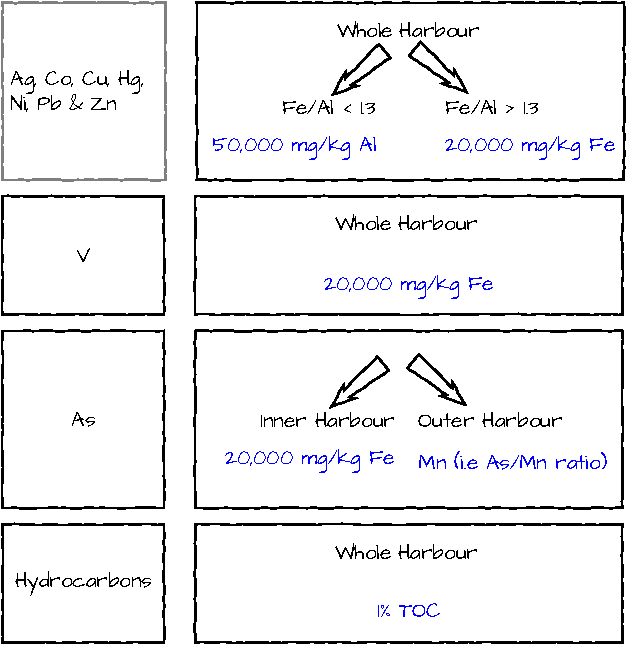
\includegraphics{manual_files/figure-pdf/fig-standardisations-1.pdf}

}

\caption{\label{fig-standardisations}Diagram illustrating the
standardisation (normalisation) rules applied to each variable. In each
case, the text in blue represents the appropriate divisor used in the
standardisation.}

\end{figure}%

\subsubsection{Create site lookup}\label{create-site-lookup}

This task creates a lookup that maps sites to zones.

\subsection{Stage 4 - Exploratory data
analysis}\label{stage-4---exploratory-data-analysis}

At the completion of this stage, the Exploratory Data Analysis menu and
Stage 5 button will become active and the Exploratory Data Analysis page
will be populated with the a range of exploratory figures. This Stage
involves numerous tasks that each prepare the data in formats conducive
to the production of the figures while navigating the Exploratory Data
Analysis page.

\subsection{Stage 5 - Temporal
analysis}\label{stage-5---temporal-analysis}

At the completion of this stage, the Analysis menu will become active
and the Analysis page will be populated with the a range of modelled
outputs.

The temporal analyses essentially involve the fitting of separate
Bayesian Hierarchical models (Gelman and Hill 2007) to the full time
series of all sites within each focal Zone. From such models (outline
below), site and zone level modelled trends can be inferred and
thereafter aggregated up to Area and Whole of Harbour level trends as
well.

The general form of the models employed is as follows:

\[
\begin{aligned}
y_{i,s} &\sim{} \Gamma(\mu_{i,s}, \phi)\\
log(\mu_{i,s}) &= (\beta_0 + \gamma_{s[i],0}) + \sum_{j=1}^nT_{[i],j}.(\beta_j + \gamma_{s[i],j]})\\
\phi&\sim\Gamma(0.01, 0.01)\\
\beta_0&\sim{}\mathit{t}(3, \alpha_1, \alpha_2)\\
\beta_{[1,n]}&\sim{}\mathit{t}(3, 0, \alpha_3)\\
\gamma_{[1..p]}&\sim{}MVN(0, \boldsymbol{\Sigma_s})\\
\boldsymbol{\Sigma_s} &=
{\begin{pmatrix}
\sigma_{s_1}^2 & \rho_s \sigma_{s_1} \sigma_{s_2} & \rho_s \sigma_{s_1} \sigma_{s_3}\\
\rho_s \sigma_{s_1} \sigma_{s_2} & \sigma_{s_2}^2 & \rho_s \sigma_{s_2} \sigma_{s_3}\\
\rho_s \sigma_{s_1} \sigma_{s_3}  & \rho_s \sigma_{s_2} \sigma_{s_3} & \sigma_{s_3}^2
\end{pmatrix}}\\
\sigma_{s[1,2,3]} &\sim \mathit{t}(3, 0, \alpha_2)\\
\rho_s &\sim \mathit{LKJcorr}(1)\\
\end{aligned}
\]

The \(i_{th}\) value (\(y\)) from the \(s_{th}\) site was assumed to be
drawn from a gamma (\(\Gamma\)) distribution parameterised by a mean
(\(\mu_{i,s}\)) and dispersion (\(\phi\)) respectively. The (natural
log) expected means were described by a linear model that included an
intercept (\(\beta_0\)), varying effects of site (\(\gamma_{s,0}\)) and
annual changes in value (\(\gamma_{s,j}\)) as well as the population
effects (\(\beta_1\)) of year (\(T\)). Weakly informative flat-t (3 df)
priors were applied to the intercept and all population effect
parameters. The values (\(\alpha_1\), \(alpha_2\) and \(\alpha_3\)) used
to define the weakly informative priors were developed from simple
summary statistics of the raw data. A weakly informative gamma prior was
applied to the dispersion parameter. The varying effects were assumed to
follow a multivariate normal with a site-specific covariance structure
whose variances follow a weakly informative flat t distribution and
whose correlation follows a LJK distribution with parameter of 1.

When the data include values that are below the limit of detection, the
model outlined above is modified so as to apply left censoring.

All Bayesian models were fit using the \texttt{brms} (Bürkner 2017)
package within the R Graphical and Statistical Environment (R Core Team
2024). All models had an adaptive delta of 0.95 and had three chains,
each with 5000 no-u-turn (NUTS) iterations, a warmup of 1000 and a
thinning rate of 5.

Separate models are fit to each variable, for each appropriate
standardisation type, for each zone. At the time of writing this manual,
this equates to nearly 300 models.

\subsubsection{Retrieve data}\label{retrieve-data-1}

This task literally just reads in the data stored at the end of the
previous stage.

\subsubsection{Prepare data}\label{prepare-data}

This task ensures that the data are formatted and packaged up into sets
associated with each individual model.

\subsubsection{Prepare priors}\label{prepare-priors}

This task is responsible for defining weakly informative priors on all
parameters for each model. The priors associated with the model for a
specific variable/zone were developed by taking simple summary
statistics of the mean, median, standard deviation and median absolute
deviation of the log of the values conditional on year.

\begin{itemize}
\tightlist
\item
  \(\alpha_1\) was taken from the median of the log values from the
  first sampling year. This was used as the mean of the model intercept
  (\(\beta_0\)) prior
\item
  \(\alpha_2\) was taken from the maximum of the median absolute
  deviations of log values for each sampling year. This was used as the
  standard deviation for the model intercept (\(\beta_0\)) as well as
  the standard deviation for the variances (\(\sigma_s\)) of the varying
  effects.
\item
  \(\alpha_3\) was taken as the maximum of the difference in mean log
  values between years and this was used to inform the standard
  deviation of the population effect (\(\beta\)) priors.
\end{itemize}

\subsubsection{Prepare model template}\label{prepare-model-template}

This task essentially involves compiling a single simple model to use as
a template for most other models. Model compilation consumes
approximately 40 seconds of time prior to the model running. Since most
of the models are the same (only the priors and the data differ), and
this project requires the fitting of a very large number of models, the
use of a pre-compiled template can speed up the overall modell fitting
process dramatically.

\subsubsection{Fit models}\label{fit-models}

This task involves fitting all combinations of the models. As each new
model is fit, the \textbf{Model Logs* pane of the }Dashboard** page will
be updated with a running progress (model number out of a total),
zone/variable/standardisation name along with a message indicating
whether the model was run or retrieved from a previous run. Each single
model is expected to take approximately 1 minute to run (depending on
the clock speed of the computer) so adjust your expectations
accordingly.

\subsubsection{Validate models}\label{validate-models}

This task will perform a range of model validation checks and assign
flags against models that display sub-optimal characteristics. Similar
to the model fitting task, the status of validation can be tracked in
the \textbf{Model Log} pane of the \textbf{Dashboard} page. Details of
the validations performed are given in section
Section~\ref{sec-validation}.

\subsubsection{Compile zone results}\label{compile-zone-results}

This task will extract posteriors and summaries for model derived cell
means (estimates for each year) for each zone along with effects
(comparisons between sets of years). With respect to the effects, the
comparisons are:

\begin{itemize}
\tightlist
\item
  Baseline to each subsequent year
\item
  Most recent year to the year prior to that
\end{itemize}

The full posteriors of each of the above are stored in files to be
accessed from the \textbf{Analysis} page.

\subsubsection{Collect zone results}\label{collect-zone-results}

This task collects file pointers across all models together into a
single file for more convenient access in the \textbf{Data} page.

\subsubsection{Compile site results}\label{compile-site-results}

Similar to the \textbf{Compile zone results} this task extracts
posteriors and summaries for model derived cell means (estimates for
each year) for each site along with effects (comparisons between sets of
years). With respect to the effects, the comparisons are:

\begin{itemize}
\tightlist
\item
  Baseline to each subsequent year
\item
  Most recent year to the year prior to that
\end{itemize}

The full posteriors of each of the above are stored in files to be
accessed from the \textbf{Analysis} page.

\subsubsection{Collect site results}\label{collect-site-results}

This task collects file pointers across all models together into a
single file for more convenient access in the \textbf{Data} page.

\subsubsection{Compile area results}\label{compile-area-results}

This task aggregates the zone level posteriors together before
re-calculating the cell means and effects.

\subsubsection{Collect area results}\label{collect-area-results}

This task collects file pointers across all models together into a
single file for more convenient access in the \textbf{Data} page.

Finally all site, zone and area results are concatenated together into a
single file.

\section{App pages}\label{app-pages}

\subsection{Landing page}\label{sec-landing}

To run this tool, please adhere to the following steps:

\begin{enumerate}
\def\labelenumi{\arabic{enumi}.}
\tightlist
\item
  review the \emph{Path Settings} (specifically checking the
  \textbf{``Data input dir''} and ensuring that there is at least one
  data file listed in the box under this setting
\item
  review the \emph{Run Settings}. In particular,

  \begin{itemize}
  \tightlist
  \item
    consider whether you need to \textbf{Clear the previous data} -
    clicking the button to do so. Clearing the previous data deletes all
    cache and ensure that the analyses are performed fresh. \textbf{This
    is recommended whenever the input data changes}. Not clearing the
    previous data allows the user to skip directly to later run stages
    if earlier stages have already been run.
  \item
    consider the Limit of Reporting (LoR) setting.

    \begin{itemize}
    \tightlist
    \item
      the default is to set the value equal to the specified limit of
      reporting for a value (such values must start with a
      ``\textless{}'') and will be flagged as ``left'' censored. Models
      that accommodate censored data take a probabilistic approach to
      inferring the likely distribution of all observations including
      those beyond the limit of reporting and are considered more
      appropriate.
    \item
      the alternative is the more traditional approach of replacing the
      value with 1/2 of the limit of reporting value and using this in
      the analyses. Whilst traditional, this approach tends to make the
      resulting values into outliers and thus problematic in analyses.
    \end{itemize}
  \end{itemize}
\item
  navigate the \emph{Dashboard} via the menu on the left sidebar
\end{enumerate}

\subsection{Dashboard}\label{sec-dashboard}

The analysis pipeline comprises numerous \textbf{Stages}, each of which
is made up of several more specific \textbf{Tasks}. The individual Tasks
represent an action performed in furtherance of the analysis and of
which there are reportable diagnostics. For example, once the
application loads, the first Stage of the pipeline is to prepare the
environment. The first Task in this Stage is to load the necessary R
packages used by the codebase. Whilst technically, this action consists
of numerous R calls (one for each package that needs to be loaded), the
block of actions are evaluated as a set.

Initially, all upcoming tasks are reported as ``pending'' ({}). As the
pipeline progresses, each Task is evaluated and a status is returned as
either ``success'' ({}) or ``failure'' ({}).

The Stage that is currently (or most recently) being run will be
expanded, whereas all other Stages will be collapsed (unless they
contain errors). It is also possible to expand/collapse a Stage by
double clicking on its title (or the small arrow symbol at the left side
of the tree).

As the pipeline progresses, Task logs are written to a log file and
echoed to the \textbf{Logs} panel. Each row represents the returned
status of a specific Task and are formatted as:

\begin{itemize}
\tightlist
\item
  the time/date that the Task was evaluated
\item
  the Task status, which can be one of:

  \begin{itemize}
  \tightlist
  \item
    \texttt{SUCCESS} the task succeeded
  \item
    \texttt{FAILURE} the task failed and should be investigated
  \item
    \texttt{WARNING} the task contained a warning - typically these can
    be ignored as they are usually passed on from underlying routines
    and are more targetted to developers than users.
  \end{itemize}
\item
  the Stage followed by the Task name
\item
  in the case of errors and warnings, there will also be the error or
  warning message passed on from the underlying routines. These can be
  useful for helping to diagnose the source and cause of issues.
\end{itemize}

The Logs in the Log panel are presented in chronological order and will
autoscroll such that the most recent log is at the bottom of the
display. If the number of Log lines exceeds 10, a scroll bar will appear
on the right side of the panel to help reviewing earlier Logs.

\begin{tcolorbox}[enhanced jigsaw, toprule=.15mm, rightrule=.15mm, opacityback=0, bottomrule=.15mm, colback=white, breakable, left=2mm, arc=.35mm, leftrule=.75mm, colframe=quarto-callout-color-frame]

Note

The Status and Logs are completely refreshed each time the application
is restarted.

\end{tcolorbox}

The Progress panel also has a tab (called \textbf{Terminal-like}) which
provides an alternative representation of the status and progress of the
pipeline.

Under the \textbf{Logs} panel, there is a \textbf{Model Logs} panel.
This panel provides additional status and progress about the fitting and
processing of individual statistical models.

\subsection{Data}\label{sec-data}

The Data page comprises two panels or subpages accessable by tabs named
``Raw data'' and ``Processed data'' at the top of the page.

\begin{tcolorbox}[enhanced jigsaw, toprule=.15mm, opacityback=0, colbacktitle=quarto-callout-note-color!10!white, colback=white, breakable, opacitybacktitle=0.6, toptitle=1mm, colframe=quarto-callout-note-color-frame, title=\textcolor{quarto-callout-note-color}{\faInfo}\hspace{0.5em}{Note}, rightrule=.15mm, leftrule=.75mm, bottomrule=.15mm, left=2mm, bottomtitle=1mm, coltitle=black, titlerule=0mm, arc=.35mm]

The contents of the Processed data subpage will not be revealed until
the completion of Stage 3.

\end{tcolorbox}

\subsubsection{Raw data panel}\label{raw-data-panel}

The \textbf{Raw data} panel displays the input data and associated
validation summaries (once the data have been loaded - that is, once
Stage 2 has been complete). The table above initially has a row for each
of the input files.

The title of each input file name is displayed in the first column
(\textbf{File}). The size and file creation time in the next two columns
(fields). The \textbf{Sheet} field lists the parsed sheets within the
excel file and the \textbf{Status} column indicates whether all the
sheets are valid ({}) or not ({}).

To the left of the file name there is a black triangle. This is an
content expansion marker. When the triangle points to the right,
clicking anywhere in the cell containing the triangle will expand the
table to reveal additional rows (one for each of the sheets in that
excel file). The rows can be collapsed again by clicking on the cell
containing the downward pointing triangle.

When the additional rows are visible, the \textbf{Status} field icons
indicate whether the sheet was valid ({}) or not ({}).

Clicking on the cell containing the name for a Sheet will make this the
\emph{focal} Sheet of the \textbf{Data} and \textbf{Validation} tabs:

\begin{itemize}
\item
  the table in the \textbf{Data} tab displays the \emph{focal} content
  of the input data Sheet. Only the first 10 rows are displayed in the
  table, the others being accessable via the controls under the table.

  Note, all numerical values are displayed only to three decimal places,
  yet the actual underlying data is full resolution.
\item
  the table in the \textbf{Validation} tab displays more details about
  which fields or rows of the \emph{focal} Sheet failed validation
  tests.

  If there were no validation issues, this table will be empty.
  Otherwise, the description field will indicate the nature of the
  violation and in the case of issues with an individual record, the
  offending row will be presented across the remaining cells in the row.
  For more information about the validation tests, please refer to the
  \textbf{Data requirements} box (to the right of this box in the app).
\end{itemize}

Underneath both the Data and Validation tables, there is a
\textbf{Download as csv} button. Via this button, you can download a
comma separated text file version of the data in the table for further
review in a spreadsheet of your choice. Once you click this button, you
will be prompted to navigate to a suitable location to store the file.

\subsubsection{Processed data panel}\label{processed-data-panel}

The Processed data panel displays the first 10 rows of the complete,
compiled and processed data set. Descriptions of each field of these
data are provided in the table below.

\begin{tcolorbox}[enhanced jigsaw, toprule=.15mm, opacityback=0, colbacktitle=quarto-callout-note-color!10!white, colback=white, breakable, opacitybacktitle=0.6, toptitle=1mm, colframe=quarto-callout-note-color-frame, title=\textcolor{quarto-callout-note-color}{\faInfo}\hspace{0.5em}{Note}, rightrule=.15mm, leftrule=.75mm, bottomrule=.15mm, left=2mm, bottomtitle=1mm, coltitle=black, titlerule=0mm, arc=.35mm]

This panel will not become active until the completion of Stage 3.

\end{tcolorbox}

The \textbf{Processed data} panel displays the processed data. As part
of the processing, the following new fields will be created:

\begin{longtable}[]{@{}
  >{\raggedright\arraybackslash}p{(\columnwidth - 2\tabcolsep) * \real{0.2000}}
  >{\raggedright\arraybackslash}p{(\columnwidth - 2\tabcolsep) * \real{0.8000}}@{}}
\toprule\noalign{}
\begin{minipage}[b]{\linewidth}\raggedright
Field
\end{minipage} & \begin{minipage}[b]{\linewidth}\raggedright
Description
\end{minipage} \\
\midrule\noalign{}
\endhead
\bottomrule\noalign{}
\endlastfoot
Sample\_key & this is a unique ID for each sample and is created as the
combination of \texttt{Sample\_ID}, \texttt{Acquired\_date\_time} and
any replicate/duplicate tokens in the \texttt{Sample\_ID} \\
*¹ (mg/kg) & observed concentration of metal in sediment sample \\
Type & whether the record pertains to a metal or hydrocarbon \\
Year\_cal & calendar year of sample collection \\
Year\_fiscal & financial year of sample collection \\
Year\_water & water year (1st Oct - 30 Sept) of sample collection \\
Year & calendar year of sample collection \\
Baseline & whether the record is a baseline record (TRUE) or not
(FALSE) \\
ZoneName & name of the Darwin Harbour Zone \\
Region & Darwin Harbour Region number \\
RegionName & name of the Darwin Harbour Region \\
Zone & Darwin Harbour Zone number \\
Area & Darwin Harbour Area (Inner or Outer) \\
Site & ID of the sampling site \\
Var & name of the measurement \\
Values & the observed measurement \\
Value\_type & whether the value is a standardised value or not \\
Fe/Al & Fe:Al where appropriate \\
Fe\_Al\_normalisation & what the sample \textbf{would be} normalised
against Fe or Al (or not applicable) if it could be normalised \\
Normalised against & what the sample \textbf{was} normalised against (if
it was normalised) \\
Normalisation flag & whether the normalisation has switched between Fe
and Al over time for this site \\
\end{longtable}

Under the column (field) headings in the Processed data panel table,
there are input boxes that act as filters. The data presented in the
table will be refined to just those cases that match the input string as
it is being typed. It is possible to engage with any or all of these
filters to help refine the search.

Under the table there is a \textbf{Download as csv} button. Via this
button, you can download a comma separated text file version of the data
in the table for further review in a spreadsheet of your choice. Once
you click this button, you will be prompted to navigate to a suitable
location to store the file.

\subsection{Exploratory Data Analysis}\label{exploratory-data-analysis}

The Exploratory Data Analysis page comprises four panels or subpages
accessable by tabs at the top of the page and named ``Temporal'',
``Temporal Type'', ``Temporal Site'' and ``Spatial Type''.

\subsubsection{Temporal}\label{temporal}

This page displays a multi-panel figure depicting the temporal sampling
design of the data within each of the Harbour Zones. The y-axis (rows)
of the figure represents the Sampling sites (based on the Site names
they were first assigned). Blue points represent the samples collected
that are considered to be ``Baseline'' or ``Reference'' samples from
which subsequent samples at the corresponding site are to be gauged
(compared). Red points represent non-``Baseline'' samples. Points are
jointed by lines to help identify discontinued sampling (where no line
exists) and where no Baselines have been defined (when the left point of
a sequence is red).

To keep the figure to a manageable size and degree of clutter, the
figure fucusses only on ``Sites'' that were first monitored in the
semester indicated by the dark blue selector to the left side of the
figure. The selectors are partitioned into 6 monthly (a semester) chunks
and clicking on a different selector will update the figure to a
different fraction of the data.

\subsubsection{Temporal Type}\label{temporal-type}

The multi-panel figure displayed on this page partitions the data into
Zone/Measurement types (via left hand selectors) and figure columns
(measures). The x-axis (rows) of the figure represents the sampling
years and the y-axis represents the individual sampling sites. Blue
points represent the samples collected that are considered to be
``Baseline'' or ``Reference'' samples from which subsequent samples at
the corresponding site are to be gauged (compared). Red points represent
non-``Baseline'' samples.

\subsubsection{Temporal Site}\label{temporal-site}

This page provides a way of fully exploring the un-modelled temporal
trends in both raw and standardised data for each Site, Measurement Type
and Variable.

Blue points represent the samples collected that are considered
``Baseline'' or ``Reference'' samples from which subsequent samples at
the corresponding site are gauged. Red points represent non-``Baseline''
samples. Multiple panels (if present) distinguish standardised and
unstandardised data. Hovering over the points will reveal some of the
pertinent underlying data associated with the point.

Different combinations of Sites, Measurement Type and Variables can be
selected via their respective dropdown boxed in the panel above the
figures.

\subsubsection{Spatial Type}\label{spatial-type}

This page provides a way to visualise the spatial distribution of
un-modelled data on a map. It also provides a representation of the
temporal trends in the data. The subset of data presented in the
temporal graph and on the map are controlled by a set of dropdown
selector boxes. The data presented on the map are also further refined
to a single year and that is controlled by the slider situated above the
temporal figure.

In the temporal figure, each point represents an individual observation
and observations collected from the same sites over time are connected
by gray lines. Blue points represent the samples collected that are
considered ``Baseline'' or ``Reference'' samples from which subsequent
samples at the corresponding site are gauged. Red points represent
non-``Baseline'' samples. Multiple panels (if present) distinguish
standardised and unstandardised data. Hovering over the points will
reveal some of the pertinent underlying data associated with the point.

Sites are represented on the map by circular points, the colour of which
are mapped to a scale proportional to the data values. Panning and
zooming of the map is done via the mouse (moving while left mouse press:
panning, scrolling of mouse button: zooming). The Zone selector dropdown
controls which Harbour Zone(s) are highlighted and populated with data.

\subsection{Analysis}\label{analysis}

The Analysis page comprises three panels or subpages accessable by tabs
at the top of the page and named ``Analysis overview'', ``Model
diagnostics'' and ``Analysis details''.

\subsubsection{Analysis overview}\label{analysis-overview}

The main feature of this panel is a table representing a very high level
overview of the results conditional on spatial scale (Site, Zone, Area),
Measurement Type (hydrocarbons or metals), Value Type (Unstandardised or
Standardised), Normalisation (Standardisation) method, Focal Year and
Contrast (each of which is controlled via a dropdown).

The table presents a matrix in which:

\begin{itemize}
\item
  the columns represent the variables
\item
  the rows represent the sites/zones/areas
\item
  the colour of the cells represents the polarity and evidence of
  change:

  \begin{itemize}
  \tightlist
  \item
    red: strong evidence of an increase
  \item
    orange: evidence of an increase
  \item
    yellow: weak evidence of an increase
  \item
    white: no evidence of change
  \item
    light green: weak evidence of a decline
  \item
    mid green: evidence of a decline
  \item
    dark green: strong evidence of a decline
  \item
    gray: model not completed (typically due to a lack of data)
  \end{itemize}
\item
  models built on data that includes values below limit of
  reporting/detection are marked with a black flag ({})
\end{itemize}

The selectors can be used to filter what subset of data are presented in
the table:

\begin{itemize}
\tightlist
\item
  scale of aggregation (site/zone/area)
\item
  whether or not the data are standardised
\item
  the type of variable (metals, hydrocarbons or both)
\item
  the focal year to compare to the baseline (2019/2020)
\end{itemize}

At the top of this page there is a collapsed box containing an overview
of the model validation checks. To view the table, ensure that the box
is expanded (click on the ``-'' icon in the upper right corner of the
box banner).

The table is filterable (by entering text in the text boxes between the
column headings and first row of data). Each row represents the
inforation about a single model. The validity tests represent whether
there is any evidence to reject (p-value \textless{} 0.05). A value of
``fail'' indicates that there is evidence that the test revealed
evidence to invalidate the assumption:

\begin{itemize}
\tightlist
\item
  \textbf{ks} the KS (uniformity test)
\item
  \textbf{ds.p} the dispersion test
\item
  \textbf{q} residual plot quantiles
\item
  \textbf{o} outlier observations
\item
  \textbf{valid} whether any of the above failed
\end{itemize}

The table is initially sorted such models flagged as potentially invalid
are towards the top.

The page also displays diagnostics and summaries of each of the fitted
models accessible via hierarchical tabs and selectable via Zone,
Variable and Standardisation selection boxes.

More information about each of the validation and summarisations are
provided inside the corresponding set of tabs.

\subsubsection{Model diagnostics}\label{model-diagnostics}

This panel displays a wide range of MCMC sampling and model validation
diagnostics as well as simple model summaries.

\paragraph{Model Validation}\label{sec-validation}

\subparagraph{Prior vs Posterior}\label{prior-vs-posterior}

Plots of priors (black points and whiskers) and posteriors (coloured
points and whiskers) for each of the main model parameters. This sort of
figure provides a way to visualy assess how \textbf{informative} the
priors are likely to be in determining the posteriors. Ideally, we want
the priors to only be \textbf{weakly} informative. That is, we only want
them to have a regularising influence (encouraging the sampler to stay
within a range of parameter estimates that are vaguely plausible).
Hence, the ideal is for the priors (black) to be either substantially
wider (longer in the figure) or centered at a different location
(position along y-axis) than the corresponding posteriors (coloured).

\subparagraph{Traceplots}\label{traceplots}

MCMC traceplots are visual tools used to assess the convergence and
mixing behavior of Markov Chain Monte Carlo (MCMC) algorithms in
Bayesian statistics. They offer valuable insights into the efficiency
and reliability of your MCMC analysis.

\textbf{What do they show?}

Each trace plot displays the values of a specific parameter estimated by
the MCMC algorithm across all iterations. Multiple parameters can be
plotted individually or jointly to compare their behavior.

\textbf{How to interpret them:}

\begin{itemize}
\item
  \textbf{Convergence:}

  A well-converged chain should exhibit stability over iterations,
  meaning the trace plot plateaus around a constant value or fluctuates
  within a predictable range. Trends or drifts indicate the chain hasn't
  converged, and the estimates might be biased.
\item
  \textbf{Mixing:}

  Good mixing implies the chain explores the parameter space
  efficiently, visiting different possible values frequently. Stuck
  chains remain in specific regions, leading to poor exploration and
  unreliable estimates.
\item
  \textbf{Autocorrelation:}

  If consecutive values in the trace plot are highly correlated, the
  chain mixes slowly, impacting efficiency.
\item
  \textbf{Mixing across chains:}

  Running multiple chains (starting from different points) should
  converge to similar values, supporting mixing and reliability.
\end{itemize}

\textbf{Interpretation tips:}

\begin{itemize}
\tightlist
\item
  Consider the expected behavior of your model: some parameters might
  naturally fluctuate more than others.
\item
  Use reference values or theoretical limits to judge if the parameter
  values seem reasonable.
\item
  Combine trace plots with other diagnostics like Gelman-Rubin
  convergence measures for a comprehensive assessment.
\end{itemize}

\subparagraph{Autocorrelation plots}\label{autocorrelation-plots}

MCMC autocorrelation plots, are another essential tool for diagnosing
the convergence and mixing of your MCMC algorithm in Bayesian
statistics.

\textbf{What are they?}

Autocorrelation plots measure the correlation between values of a
parameter at different lags (distances) within the MCMC chain. They
typically display the correlation coefficient at each lag, plotted
against the lag number. The first bar represents the correlation of MCMC
samples with themselves, and thus will always be 1 on the y-axis.

\textbf{How to interpret them:}

\begin{itemize}
\item
  \textbf{Bias:}

  The autocorrelation plot helps assess how quickly the correlation
  between samples decays as the lag increases. Ideally, samples
  collected from any process (including MCMC sampling) should all be
  independent and unbiased in order to provide unbiased estimates. If
  the autocorrelation values decay rapidly to zero as the lag increases,
  it indicates that the MCMC samples are likely to be independent and
  unbiased. Conversely, if high autocorrelation persists with large
  lags, it is possible that the MCMC samples are biased towards
  particular regions of the parameter space. **Ideally, the degree of
  autocorrelation should drop to below 0.25 by the second bar (second
  lag).
\item
  \textbf{Convergence:}

  \begin{itemize}
  \item
    Rapidly decaying autocorrelation: As the lag increases, the
    correlation between values drops quickly, indicating good
    convergence. The chain efficiently moves through the parameter
    space, providing reliable and unbiased estimates.
  \item
    High autocorrelation even at large lags: This suggests the chain is
    ``stuck'' in certain regions, not exploring the parameter space
    well. Estimates might be biased and unreliable.
  \end{itemize}
\item
  \textbf{Mixing:}

  \begin{itemize}
  \item
    High autocorrelation at small lags: The chain takes many iterations
    to ``forget'' past values, indicating slow mixing. The algorithm
    might not be efficiently exploring the parameter space.
  \item
    Autocorrelation dropping to zero around medium lags: This suggests
    the chain mixes reasonably well, considering the natural dependence
    between consecutive values.
  \end{itemize}
\end{itemize}

If autocorrelation patterns exist in the MCMC samples, the MCMC samples
should be thinned to a higher degree.

\subparagraph{Rhat plots}\label{rhat-plots}

Rhat plots, also known as Gelman-Rubin convergence diagnostic plots, are
graphical tools used to assess the convergence of multiple chains in a
Bayesian analysis. These plots are based on the Gelman-Rubin statistic
(Rhat), which compares the variance within chains to the variance
between chains.

\textbf{What are they?}

Rhat represents a ``potential scale reduction factor'', and compares the
within-chain and between-chain variances of parameter estimates from
multiple MCMC chains. It's used to assess whether the chains have mixed
well and converged to the same target distribution.

Rhat plots visualise the Rhat statistic for each parameter estimated in
the Bayesian analysis. Each parameter has its own Rhat value, and the
plot typically displayed as histograms.

\textbf{How to interpret them:}

\begin{itemize}
\item
  \textbf{Rhat \textless{} 1.01:}

  Generally indicates very good convergence, suggesting the chains have
  explored the target distribution efficiently and reached similar
  conclusions.
\item
  \textbf{Rhat \textless{} 1.05:}

  Generally indicates acceptable convergence.
\item
  \textbf{Rhat \textgreater{} 1.05:}

  Indicates significant convergence problems, meaning the chains haven't
  mixed well and could lead to biased estimates. It implies that at
  least one of the chains may have traversed different features of the
  parameter space compared to the other chain(s). If so, then there may
  well be other additional un-traversed features. It is possible that
  the MCMC sampler may not have fully explored all important regions of
  the parameter space.
\end{itemize}

\subparagraph{Effective Sample Size}\label{effective-sample-size}

ESS plots, or Effective Sample Size plots, are graphical tools used to
assess the effective sample size of MCMC samples obtained from Bayesian
analyses. The effective sample size quantifies the amount of independent
information contained in the MCMC samples and is crucial for accurate
estimation of posterior quantities.

\textbf{How do they work?}

Imagine your MCMC chain has length \(n\), but due to autocorrelation,
not all \(n\) iterations provide truly independent information. ESS
attempts to quantify this by estimating the number of independent
samples equivalent to your chain, effectively capturing the information
content.

\textbf{How to interpret them:}

\begin{itemize}
\item
  \textbf{High ESS (closer to \(n\)):}

  This indicates good efficiency, meaning your chain efficiently
  explores the parameter space and provides reliable estimates.
\item
  \textbf{Low ESS (much smaller than \(n\)):}

  Suggests poor efficiency, with high autocorrelation reducing the
  effective number of independent samples. This can lead to wider
  credible intervals and less precise estimates.
\end{itemize}

In order to have enough MCMC samples to provide meaningful summaries,
each parameter should have at least 1000 effective samples.

The ESS values are often expressed as fractions of the total \(n\) and
represented graphically as a histogram. Ideally, most (if not all) the
ESS values should be above 0.5.

If there are low ESS, it suggests that either the total number of
iterations was not large enough or the sampler was not sampling
efficiently. For the former case, the sampler should be re-run with
additional iterations. In the later case, it is likely that the model
itself (or the priors) are mis-specified and this should be addressed
before rerunning the model.

\subparagraph{Posterior Probability
plots}\label{posterior-probability-plots}

Posterior probability density overlay plots display the density
distribution of the observed data (dark line) overlayed upon the density
distributions of a large number of posterior predictions (fainter blue
lines).

The general idea is that if a model is to be useful, it should be able
to generate observations (predictions) that approximate the data used to
train the model in the first place. If this is not the case, then it is
likely that the model does not adequately capture the pertinent
properties of the observed data.

Ideally, the densities of the numerous realisations from the posteriors
should match closely the density of the original observed data. The
manner by which the densities differ from that of the original data can
be used to infer what aspects of the data the model is under or over
estimating and adjustments can be made to the model accordingly.

\subparagraph{Simulated (DHARMa)
residuals}\label{simulated-dharma-residuals}

Since statistical models are low dimensional representations of a system
the reliability of a statistical model will depend on the degree to
which certain assumptions are met. Many of these assumptions can be
explored by examination of the model residuals.

Patterns in residuals suggest either issues of dependencies (biases),
poor model structure and a general lack of model fit. However, for many
statistical models, discerning genuinely violation-indicating patterns
in residuals from artifacts due to the model type can be really
difficult - if not impossible.

Within R, the \emph{DHARMa} (Diagnostics for HierArchical Regression
Models: Hartig (2022)) package generates standardised residuals via
simulation and uses these as the basis of a range of tools to diagnose
common modelling issues including outliers, heterogeneity,
over-dispersion, autocorrelation.

New observations simulated from the fitted model are used to calculate a
cumulative density function (CDF) that describes the probability profile
of each observation. Thereafter, the residual of an observation is
calculated as the value of the CDF that corresponds to the actual
observed value:

\begin{itemize}
\tightlist
\item
  a value of 0 indicates that the observed value was less than all
  simulated values
\item
  a value of 1 indicates that the observed value was greater than all
  simulated values
\item
  a value of 0.5 indicates that the probability of obtaining the
  observed value is 50\%.
\end{itemize}

This approach ensures that all residuals have the same interpretation
irrespective of the model and distribution selected.

\emph{DHARMa} supports a variety of diagnostic plots based on the
simulated residuals, including residual plots, QQ plots, and test-based
diagnostic plots. These plots allow for visual inspection of model
adequacy and can reveal patterns or deviations indicative of model
misspecification or violation of assumptions. The most common plots and
their interpretations are:

\begin{itemize}
\item
  a \textbf{Q-Q plot}

  Ideally all points should be close to the diagonal red line. Overlayed
  onto this plot are three additional tests.

  \begin{enumerate}
  \def\labelenumi{\arabic{enumi}.}
  \tightlist
  \item
    KS (Kolmogorov-Smirnov) test investigates whether the (in this case
    simulated) are likely to have been drawn from the nominated
    distribution.
  \item
    Dispersion test investigates whether the is any evidence of
    overdispersion (more variability than the model expects) estimated
    as the standard deviation of the data is equal to that of the
    simulated data)
  \item
    Outlier test investigates for the prevalence of outliers (when
    observed values are outside the simulated range)
  \end{enumerate}
\item
  a \textbf{Residual vs Predicted plot}

  Ideally, there should be no patterns in the residuals. To help
  identify any patterns, quantile trends are overlayed. Ideally, there
  should be a flat black line at each of the quantiles of 0.25, 0.5 and
  0.75. In some circumstances, quantiles cannot be computed and in such
  cases a single dashed smoother many be placed over the data cloud.
\item
  a \textbf{Dispersion plot}

  The observed model dispersion is overlayed (red line) upon the
  distribution (black) of simulated dispersion values. Ideally the red
  line should be in the middle of the simulated distribution.

  \begin{itemize}
  \tightlist
  \item
    If the red line is to the far right, the model is considered
    overdispersed. Parameter uncertainty is typically underestimated in
    overdispersed models - this leads us to be more confident in our
    results than we should be and this is bad.
  \item
    If the red line is to the far left, the model is considered
    underdispersed. This is usually an artifact and results in our
    estimates being more conservative than they perhaps should be.
    Underdispersion is less of an issue as it just results in more
    conservatism in results.
  \end{itemize}
\end{itemize}

\textbf{Note}, the individual tests that accompany the diagnostic plots
tend to be stricter than the assumptions we are seeking to explore. That
is, statistical models tend to be reasonably robust to mild assumption
violations, yet the diagnostic tests are fairly strict. Hence, the tests
are used to flag potential issues, yet the ownace is still on the
researchers to explore these violations in greater detail and evaluate
whether they are likely to have any important consequences.

\paragraph{Model Summaries}\label{model-summaries}

The coefficients (parameter estimates) table displays each of the main
model parameter estimates on the scale of the link function. Parameters
that start with \texttt{b\_} are the population-level (fixed) effects.
Parameters that start with \texttt{sd\_} are the varying (random)
effects.

The table lists the posterior median as well as lower and upper bounds
of the 95\% Highest Posterior Density (HPD) interval for each parameter.
Also tabulated are the total number of posterior draws
(\texttt{length}), Rhat values (\texttt{rhat}), and effective sample
size in both the bulk of the posterior (\texttt{ess\_bulk}) and tail of
the posterior (\texttt{ess\_tail}).

\subsubsection{Analysis details}\label{analysis-details}

This panel has two sub-panels for displaying ``Modelled trends'' and
``Modelled effects''.

\paragraph{Modelled trends}\label{modelled-trends}

The modelled (predicted) values of a focal variable are displayed in
tabular and graphical form.

In the table, each row represents the summaries of predictions for a
specific year. The summaries are in the form of median as well as lower
and upper 95\% highest probability density (HPD) intervals of the full
model posteriors. Years in which data included values below the limit of
reporting are marked by a black flag ({}). The table also indicates
which years are considered Baseline.

These same summaries are also presented graphically in the figure.
Additionally, the figure displays the underlying un-modelled data in
gray. Individual sites are connected by gray lines.

\paragraph{Modelled effects}\label{modelled-effects}

This table summarises the comparisons between the average of the
baseline year(s) and each of the subsequent reporting years. Values are
reported on a \textbf{fold} (fractional) scale. On this scale, a value
of 1 indicates no change. Values of 0.5 and 2 would indicate that the
value in the reporting year is respectively half and twice that of the
baseline year(s).

Posteriors of the comparisons are summarised by their medians as well as
the lower and upper bounds of the 95\% Highest Posterior Density (HPD)
interval. Also tabulated are the exceedence probabilities associated
with the probability that the values have declined since the baseline
year(s) (\texttt{Pl}) and the probabilities that they have increased
(\texttt{Pg}). These probabilities must sum to 1 and it is only
necessary to explore the larger value per comparison. As a guide
exeedence probabilities:

\begin{itemize}
\tightlist
\item
  \textbf{\textgreater0.95} provide strong evidence of an effect
  (change)
\item
  \textbf{\textgreater0.9} provide evidence of an effect (change)
\item
  \textbf{\textgreater0.85} provide week evidence of an effect (change)
\end{itemize}

Finally, there is also a column that represents the polarity and
evidence of change via a color.

\begin{itemize}
\tightlist
\item
  red: strong evidence of an increase
\item
  orange: evidence of an increase
\item
  yellow: weak evidence of an increase
\item
  white: no evidence of change
\item
  light green: weak evidence of a decline
\item
  mid green: evidence of a decline
\item
  dark green: strong evidence of a decline
\end{itemize}

The full modelled posteriors are depicted in the figure under the table.
The y-axis represents each of the contrasts (comparisons between sets of
years or years and the Baseline). The posterior distributions are
coloured according to the polarity and degree of evidence as outlined
above.

The full and summarised posteriors can be presented on either a
\textbf{percentage} scale (default) or \textbf{fold} scale and this is
controlled via a dropdown box above the table.

\begin{itemize}
\tightlist
\item
  the percentage scale is interpreted as the percentage change between
  the contrasting years. For example, percentage changes of -20, 20 and
  0 indicate a 20\% decline, 20\% increase and no change respectively.
\item
  the fold scale is interpreted as the fold change between the
  contrasting years. For example, fold changes of 0.5, 2 and 1 indicate
  a halving, a doubling and no change respectively.
\end{itemize}

\faIcon{thumbs-up}

\phantomsection\label{refs}
\begin{CSLReferences}{1}{0}
\bibitem[\citeproctext]{ref-brms}
Bürkner, Paul-Christian. 2017. {``{brms}: An {R} Package for {Bayesian}
Multilevel Models Using {Stan}.''} \emph{Journal of Statistical
Software} 80 (1): 1--28. \url{https://doi.org/10.18637/jss.v080.i01}.

\bibitem[\citeproctext]{ref-Gelman-2007-2007}
Gelman, A., and J. Hill. 2007. \emph{Data Analysis Using Regression and
Multilevel/Hierarchical Models}. Cambridge, UK: Cambridge University
Press.

\bibitem[\citeproctext]{ref-DHARMa}
Hartig, Florian. 2022. \emph{DHARMa: Residual Diagnostics for
Hierarchical (Multi-Level / Mixed) Regression Models}.
\url{https://CRAN.R-project.org/package=DHARMa}.

\bibitem[\citeproctext]{ref-R-2024}
R Core Team. 2024. \emph{R: A Language and Environment for Statistical
Computing}. Vienna, Austria: R Foundation for Statistical Computing.
\url{https://www.R-project.org/}.

\end{CSLReferences}




\end{document}
